\documentclass[12pt,a4paper]{tucarticle2019}

\usepackage[ngerman]{babel}
\usepackage[backend=biber, sorting=none]{biblatex}
\addbibresource{Hauptseminar.bib}
\usepackage[hidelinks]{hyperref}
\usepackage{graphicx}
\usepackage{float}
\usepackage{ragged2e}
\usepackage{listings}
\usepackage{xcolor}

\usepackage[utf8]{inputenc}
\usepackage[T1]{fontenc}
\usepackage{amsmath,amssymb}
\usepackage{stmaryrd}
\usepackage{minted}


\DeclareUnicodeCharacter{21D2}{$\Rightarrow$}
\DeclareUnicodeCharacter{2200}{$\forall$}
\DeclareUnicodeCharacter{2203}{$\exists$}
\DeclareUnicodeCharacter{2260}{$\neq$}
\DeclareUnicodeCharacter{2227}{$\land$}
\DeclareUnicodeCharacter{27F6}{$\longrightarrow$}
\DeclareUnicodeCharacter{2208}{$\in$}
\DeclareUnicodeCharacter{27F7}{$\longleftrightarrow$}
\DeclareUnicodeCharacter{2228}{$\lor$}
\DeclareUnicodeCharacter{2209}{$\notin$}
\DeclareUnicodeCharacter{222A}{$\cup$}
\DeclareUnicodeCharacter{27E6}{$\llbracket$}
\DeclareUnicodeCharacter{03BB}{$\lambda$}
\DeclareUnicodeCharacter{27E7}{$\rrbracket$}
\DeclareUnicodeCharacter{27F9}{$\Longrightarrow$}
\DeclareUnicodeCharacter{2218}{$\circ$}
\DeclareUnicodeCharacter{2500}{\texttt{-}}
\DeclareUnicodeCharacter{2261}{$\equiv$}
\DeclareUnicodeCharacter{2225}{$\parallel$}
\DeclareUnicodeCharacter{22C0}{$\bigwedge$}

\lstset{
	basicstyle=\ttfamily\small,
	keywordstyle=\color{blue},
	commentstyle=\color{gray},
	stringstyle=\color{green!50!black},
	numberstyle=\tiny,
	breaklines=true,
}
\lstset{
	basicstyle=\ttfamily\small,
	columns=fullflexible,
	keepspaces=true,
	breaklines=true,
	frame=single,
	framesep=0pt,
	numbers=left,
	numberstyle=\tiny,
	numbersep=3pt,
	xleftmargin=0pt,
	xrightmargin=0pt,
	aboveskip=1pt,
	belowskip=1pt,
	showstringspaces=false
}

\lstdefinelanguage{Isabelle}{
	keywords={lemma, theorem, proof, assume, show, have, thus, qed, by, definition, fun, where, assumes, and, shows, datatype, if, then, else, case, of, type_synonym, inductive, using, rule, moreover, ultimately, next, obtain, hence},
	sensitive=true,
	comment=[l]{--},
	morecomment=[s]{(*}{*)},
	mathescape=true,
	morestring=[b]",        % "..."
	morestring=[s]{<<}{>>}, % <<...>>
	stringstyle=\color{green!50!black}
}
\lstset{language=Isabelle}

\newcommand{\isabelle}[1]{\mintinline{isabelle}{#1}}

\newcommand{\thy}[3]{
	\inputminted[
	fontsize=\small,
	breaklines,
	linenos,
	firstline=#1,
	lastline=#2
	]{isabelle}{#3}
}
\newcommand{\thyKleppNetw}[2]{
	\thy{#1}{#2}{Hauptseminar/Kleppmann/Network.thy}
}
\newcommand{\thyKleppTupac}[2]{
	\thy{#1}{#2}{Hauptseminar/Kleppmann/Kleppmann_2PC.thy}
}
\newcommand{\thyKleppInv}[2]{
	\thy{#1}{#2}{Hauptseminar/Kleppmann/Kleppmann_inv_def.thy}
}
\newcommand{\thyKleppInvOne}[2]{
	\thy{#1}{#2}{Hauptseminar/Kleppmann/Kleppmann_inv_1.thy}
}
\newcommand{\thyKleppAc}[2]{
	\thy{#1}{#2}{Hauptseminar/Kleppmann/Kleppmann_ac.thy}
}

\newcommand{\thyIoaAsig}[2]{
	\thy{#1}{#2}{Hauptseminar/IOA/HOLCF/Asig.thy}
}
\newcommand{\thyIoaAutomata}[2]{
	\thy{#1}{#2}{Hauptseminar/IOA/HOLCF/Automata.thy}
}
\newcommand{\thyIoaTupac}[2]{
	\thy{#1}{#2}{Hauptseminar/IOA/HOLCF/Automata_2PC.thy}
}
\newcommand{\thyIoaInv}[2]{
	\thy{#1}{#2}{Hauptseminar/IOA/HOLCF/Automata_inv_def.thy}
}
\newcommand{\thyIoaInvOne}[2]{
	\thy{#1}{#2}{Hauptseminar/IOA/HOLCF/Automata_inv_1.thy}
}
\newcommand{\thyIoaAc}[2]{
	\thy{#1}{#2}{Hauptseminar/IOA/HOLCF/Automata_ac.thy}
}

\author{\\\\Sepp Stage (Matrikelnummer: 791122)\\Technische Universität Chemnitz\\Hauptseminar\\Sommersemester 2026\\Betreuer: M. Sc. Jonas Henschel}

\title{Verifikation verteilter Systeme in Isabelle: Ein Vergleich von Kleppmann und I/O-Automaten}

\begin{document}
	\justifying
	\maketitle
	\newpage
	\tableofcontents	
	\newpage
	\section{Einleitung}


	Im Januar 1990 kam es zu einem Fehler im AT\&T Kommunikationsnetz, der über 60.000 Amerikaner ohne Telefonanschluss ließ. Dieser großflächige Ausfall wurde durch eine einzelne Netzwerkkomponente in New York ausgelöst \cite{atat}.
	
	Der Ausfall und anschließende Neustart dieser Komponente führte zu Nachrichten, die von benachbarten Netzwerkkomponenten nicht korrekt gedeutet wurden, was ebenfalls zum Absturz dieser Komponenten führte \cite{atat2}. So konnte sich ein lokales Problem über das System großflächig ausbreiten.
	
	In verteilten Systemen können selbst kleine Probleme einen großen Schaden anrichten. Die Schwierigkeit besteht darin, dass kleine und seltene Fehlerkombinationen oft durch Tests alleine nicht vollständig abgedeckt werden können. Bereits kleine unvorhergesehene Abweichungen im Nachrichtenverhalten können schnell zu großflächigen Ausfällen führen.
	
	Diese Komplexität verteilter Systeme erfordert daher formale Methoden mit mathematischen Beschreibungen, welche maschinelle Verifikation ermöglichen. Dadurch kann unter den getroffenen Annahmen Korrektheit mathematisch nachgewiesen werden.
	
	Ein bekanntes Beispiel für die Schwierigkeit verteilter Koordination ist das Zwei-Phasen-Commit-Protokoll, welches Konsistenz zwischen mehreren Teilnehmern garantiert, jedoch empfindlich gegenüber Ausfällen ist \cite{kleppmannbook}.
	
	Ziel dieser Arbeit ist die formale Modellierung und Verifikation des Zwei-Phasen-Commit-Protokolls im Beweisassistenten Isabelle. Dabei werden zwei unterschiedliche Modellierungsansätze untersucht. Eine Modellierung basierend auf dem verteilten Systemmodell nach Kleppmann, und eine Darstellung mittels I/O-Automaten nach Lynch und Tuttle. 
	Das Zwei-Phasen-Commit-Protokoll wird in beiden Frameworks implementiert. Ebenfalls wird dabei die Eigenschaft der einheitlichen Zustimmung formalisiert und bewiesen. Da beide Modellierungsansätze Vor- und Nachteile hinsichtlich Nutzbarkeit, Beweisaufwand und Modularität aufweisen, werden die Implementierungen und Beweise anschließend im jeweiligen Framework analysiert und miteinander verglichen.
	
	\newpage
	\section{Das Zwei-Phasen-Commit-Protokoll}
	Dieses Kapitel beschreibt das zugrunde liegende verteilte Protokoll unabhängig von seiner formalen Darstellung. Hier wird die von Jens Lechtenbörger formalisierte Version des Protokolls zusammengefasst dargestellt \cite{tupacSpec}.
	\subsection{Problemstellung}
	Das Zwei-Phasen-Commit-Protokoll wird in verteilten Systemen eingesetzt, um alle teilnehmenden Prozesse zu einer einheitlichen Entscheidung zu führen. Dies kann beispielsweise eine Entscheidung darüber sein, ob eine Datenbanktransaktion akzeptiert und dauerhaft oder abgelehnt und rückgängig gemacht werden soll.
	\subsection{Rollen}
	Das Protokoll unterteilt die teilnehmenden Prozesse in zwei Arten. Es gibt einen Koordinator, der die letztendliche Entscheidung trifft. Der Rest der Prozesse sind die Teilnehmer \cite{tupacSpec}. Im Folgenden bezeichnet 'Prozess' einen allgemeinen Teilnehmer in einem verteilten System, während der Begriff 'Teilnehmer' speziell für einen nicht-Koordinator Prozess im Zwei-Phasen-Commit-Protokoll verwendet wird.
	\subsection{Grundlegender Ablauf}
	Der Ablauf des Protokolls wird hier anhand einer durchzuführenden Datenbanktransaktion beschrieben. Ein Übergangsdiagramm inklusive Verhalten bei Fehlern, wird in Abbildung \ref{fig:2pcAutomat} beschrieben. 
	
	Das Protokoll unterteilt sich in zwei Phasen. Die erste Phase ist die Vorbereitungsphase, wobei alle Prozesse im Initial-Zustand starten.
	Der Koordinator beginnt durch das Senden einer Prepare-Nachricht an alle Teilnehmer und wechselt in den Collecting-Zustand. Beim Erhalt einer solchen Nachricht wertet der Teilnehmer lokal aus, ob er in der Lage ist, die Transaktion durchzuführen. Ist dies der Fall, so schickt er eine Yes-Nachricht an den Koordinator zurück und wechselt in den Prepared-Zustand. Andernfalls sendet er eine No-Nachricht und geht in den Aborted-Zustand über. 
	
	Der Koordinator sammelt nun die Antworten der Teilnehmer und entscheidet daraufhin den Ablauf der zweiten Phase des Protokolls. Erhält er eine No-Nachricht, so schickt er eine Abort-Nachricht an alle Teilnehmer und wechselt in den Aborted-Zustand. Diese antworten daraufhin mit einer Ack-Nachricht und wechseln ebenfalls in den Aborted-Zustand. Sollte er stattdessen von allen Teilnehmern eine Yes-Nachricht erhalten haben, so schickt er eine Commit-Nachricht an alle Teilnehmer und wechselt in den Committed-Zustand. Diese antworten wiederum mit Ack-Nachrichten und wechseln ebenso in den Committed-Zustand.
	Sobald der Koordinator von allen Teilnehmern eine Ack-Nachricht erhalten hat, geht er in den Forgotten-Zustand über und das Protokoll ist beendet.
	
	\subsection{Protokollverhalten bei Fehlern}
	In verteilten Systemen können verschiedenste Arten an Fehlern auftreten. Diese müssen korrekt behandelt werden, um auch beim Auftreten dieser Fehler einen korrekten Ausgang des Protokolls zu gewährleisten \cite{kleppmannblog}. Dabei ist ebenfalls entscheidend, welche Fehler als möglich angenommen werden. Diese Annahmen werden als Systemannahmen bezeichnet und definieren den formalen Rahmen, innerhalb dessen ein Algorithmus modelliert und analysiert werden kann. Im Folgenden wird eine Zusammenfassung möglicher Fehlerarten in verteilten Systemen gegeben. Das Verhalten der Prozesse kann Abbildung \ref{fig:2pcAutomat} entnommen werden.
	\subsubsection{Fehlerarten in verteilten Systemen}
	Jeder Prozess in einem verteilten System kann auf verschiedenste Art und Weise mit oder ohne Warnung abstürzen \cite{lynchbook}, wobei entweder nur jegliche nicht persistente Daten verloren gehen oder gar ganze Datensätze korrumpiert werden können. Dieser Absturz kann entweder final sein oder der Teilnehmer kann erneut gestartet werden \cite{kleppmannbook}.
	
	Teilnehmer können auch byzantinisches (willkürliches) Verhalten zeigen, wobei dieses Verhalten von fehlerhaften Nachrichtensendungen bis hin zu gezielt bösartigen Handlungen reicht \cite{kleppmannbook}.
	
	Nicht nur die Teilnehmer in einem verteilten System können fehlerhaft sein, auch das zugrunde liegende Netzwerk kann Fehler aufweisen. So kann eine einzelne gesendete Nachricht verloren gehen, dupliziert werden oder eine beliebig lange Zulieferzeit aufweisen \cite{kleppmannbook}. Im schlimmsten Fall kann eine Nachricht beim Empfänger verändert ankommen, als es beim Sender abgeschickt wurde. Dabei kann zwischen erkennbar und unerkennbar geänderten Nachrichten entschieden werden. Mehrere Nachrichten können zusätzlich untereinander umgeordnet werden, sodass sie beim Empfänger in einer anderen Reihenfolge ankommen als sie beim Sender abgeschickt wurden \cite{kleppmannblog}.
	\subsubsection{Teilnehmerfehler beim Zwei-Phasen-Commit-Protokoll}
	Die hier betrachtete Version des Zwei-Phasen-Commit-Protokolls \cite{tupacSpec} betrachtet nur Abstürze von Koordinator und Teilnehmern, bei denen der persistente Speicher erhalten bleibt und lediglich nicht persistenter Speicher vollständig verloren geht. Um nach einem solchen Absturz das Protokoll korrekt fortsetzen zu können, schreibt jeder Prozess vor dem Senden einer oder mehrerer Nachrichten seinen aktuellen Zustand in den persistenten Speicher. Nach einem Absturz kann dann anhand des zuletzt geschriebenen Zustands dieser aus dem Speicher geladen werden. Dabei müssen jedoch die in diesem Zustand zu sendenden Nachrichten erneut gesendet werden.
	\subsubsection{Netzwerkfehler beim Zwei-Phasen-Commit-Protokoll}
	Neben den beschriebenen Teilnehmerausfällen behandelt dieses Zwei-Phasen-Commit-Protokoll auch Fehler im Kommunikationsnetz. Gesendete Nachrichten können verloren gehen \cite{tupacSpec}. Um damit korrekt umzugehen, wird bei jedem Senden einer oder mehrerer Nachrichten ein lokaler Timer gestartet der, sobald er abläuft, eine Sendungswiederholung jener Nachrichten auslöst. 
	Zusätzlich, sollten wiederholt die Timer des Koordinators beim Warten im Collecting-Zustand ablaufen, so bricht dieser die Entscheidung eigenständig ab und sendet Abort-Nachrichten an alle Teilnehmer.
	
	Sollte nach einer gewissen Zeit keine Prepare-Nachricht bei einem Teilnehmer ankommen, so wechselt dieser eigenständig in den Aborted-Zustand, ohne eine Nachricht zu senden.
	Bei der Implementierung dieses Protokolls werden später zusätzlich Nachrichtenduplizierung, Nachrichtenverspätung und Umordnung der Nachrichten betrachtet.
	
	
	\begin{figure}[h]
		\caption{Übergangsdiagramm für Koordinator (links) und Teilnehmer (rechts)}
		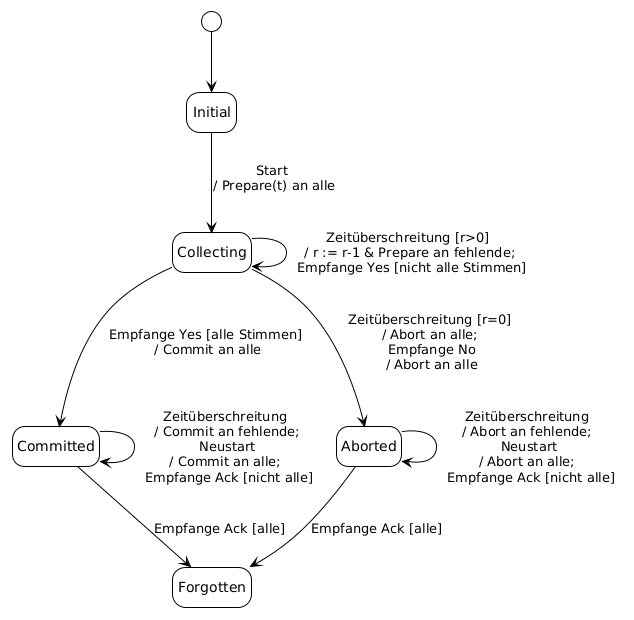
\includegraphics[width=0.5\textwidth]{Bilder/AutomatCoord}
		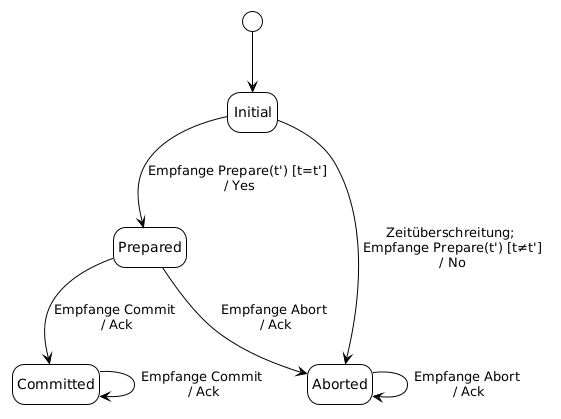
\includegraphics[width=0.5\textwidth]{Bilder/AutomatPart}
		\label{fig:2pcAutomat}
	\end{figure}
	
	\subsection{Eigenschaften}
	Eine der wichtigsten Eigenschaften, die das Zwei-Phasen-Commit-Protokoll zu jeder Zeit erfüllen muss, ist die 'einheitliche Zustimmung' \cite{kleppmannbook}. Sie besagt, dass sich alle Prozesse, die sich entscheiden, zur gleichen Entscheidung kommen müssen \cite{acSpec}. Diese Eigenschaft muss zu jeder Zeit der Ausführung des Protokolls gelten. Dies führt dazu, dass sobald sich alle Prozesse entschieden haben, eine insgesamt einheitliche Entscheidung vorliegt.
	Weitere Eigenschaft wie, dass sich alle nicht abgestürzten Prozesse irgendwann entscheiden wird hier nicht weiter betrachtet.	
	
	
	\newpage
	\section{Grundlegende Konstrukte in Isabelle}
	Isabelle ist ein interaktiver Theorembeweiser zur formalen Verifikation mathematischer Beweise. Ebenfalls können Modelle und Programme spezifiziert werden \cite{kleppmannblog}. Dieses Kapitel führt die notwendigen Isabellekonzepte ein.
	
	Funktionen können auf drei verschiedene Weisen definiert werden. Isabelle unterstützt die Lambda Notation
	\begin{minted}[
		fontsize=\small,
		breaklines,
		linenos]
		{isabelle}
	(λx. x)
	\end{minted}
	welche besonders nützlich zur ad-hoc Definition von Funktionen ist. Nicht rekursive Funktionen können mittels Definitionen wie folgt definiert werden:
	\begin{minted}[
		fontsize=\small,
		breaklines,
		linenos]
		{isabelle}
	definition sq1 :: "nat ⇒ nat" where
	"sq1 n = n*n"
	\end{minted}
	Rekursive Funktion müssen auf folgende Weise definiert werden:
	\begin{minted}[
		fontsize=\small,
		breaklines,
		linenos]
		{isabelle}
	fun sq2 :: "nat ⇒ nat" where
	"sq2 0 = 0" |
	"sq2 (Suc n) = sq2 n + 2*n + 1"
	\end{minted}
	
	Beweise können in Isabelle wie folgt geführt werden:
	\begin{minted}[
		fontsize=\small,
		breaklines,
		linenos]
		{isabelle}
	lemma sq1_eq_sq2:
	  assumes "sq1 n = s1"
	    and "sq2 n = s2"
	  shows "s1 = s2"
	  using assms
	proof(induction n arbitrary: s1 s2)
	  case 0
	  then show ?case
	    by (simp add: sq1_def)
	next
	  case (Suc n)
	  then show ?case
	    using sq1_def by fastforce
	qed
	\end{minted}
	Wobei neben \isabelle{simp} und \isabelle{fastforce} beliebige Beweistaktiken in Verbindung mit beliebigen Aussagen, wie hier \isabelle{sq1_def}, vorkommen können \cite{semantics}.
	
	Ein wichtiger Datentyp in Isabelle sind Listen. Die Leere Liste wird durch \isabelle{[]} notiert. Zwei Listen können durch den \isabelle{@}-Operator aneinander angefügt werden \cite{semantics}.
	
	Mengen können wie folgt definiert werden:
	\begin{minted}[
		fontsize=\small,
		breaklines,
		linenos]
		{isabelle}
	{} (*Leere Menge*)
	{t | x y. P}
	\end{minted}
	wobei x und y die freien Variablen im Term t sind, die in P vorkommen. \cite{semantics}.
	
	Auf Paare kann mittels der Projektionsfunktionen \isabelle{fst} und \isabelle{snd} auf das jeweils erste und zweite Element des Paares zugegriffen werden. Tupel werden als nach rechts geschachtelte Paare betrachtet. \cite{ioaHolCF}.
	Konditionale Anweisungen werden wie folgt geschrieben:
	\begin{minted}[
		fontsize=\small,
		breaklines,
		linenos]
		{isabelle}
	if P then A else C
	\end{minted}
	oder
	\begin{minted}[
		fontsize=\small,
		breaklines,
		linenos]
		{isabelle}
	case t of
	A => B |
	C => D |
	_ => E
	\end{minted}
	Diese Sprachkonstrukte bilden die Grundlage für die späteren Implementierungen.

	\newpage
	\section{Kleppmann}
	Dieses Kapitel beschreibt den ersten Modellierungsansatz, welcher von Martin Kleppmann beschrieben wurde \cite{kleppmannblog}. 
	Sein Framework, samt eines Beispielprojekts kann online gefunden werden \cite{kleppmanncode}.
	\subsection{Modellbeschreibung}
	Im Modell von Martin Kleppmann wird ein verteiltes System als eine Übergangsfunktion dargestellt, welche Ereignisse verarbeitet \cite{kleppmannblog}.
	Events werden als eigener Datentyp dargestellt, welcher einen Konstruktor für jede Eventart beinhaltet. Dieser Datentyp muss für jedes Protokoll angepasst werden, um zu definieren, was einem Prozess passieren kann.
	
	Für das hier betrachtete Zwei-Phasen-Commit-Protokoll wird dieser Datentyp wie folgt definiert:
	
	\thyKleppNetw{10}{14}
	
	Das Start-Event kann als Beginn des Protokolls verstanden werden. 
	Das Receive-Event dient zum Empfangen von Nachrichten. 
	Die Timeout- und Restart-Events dienen zum Darstellen von ablaufenden Timern, für gesendete Nachrichten und darstellen von Neustarts abgestürzter Prozesse.
	
	Der Typ einer Übergangsfunktion wird explizit definiert, um das Framework übersichtlicher zu halten.
	
	\thyKleppNetw{16}{17}
	
	Eine solche Übergangsfunktion nimmt den Prozess der das Event verarbeitet, dessen aktuellen Zustand und das zu verarbeitende Event an und gibt ein Tupel bestehend aus dem neuen Zustand des Prozesses und eine Menge, der von diesem Prozess, in diesem Schritt gesendete Nachrichten zurück \cite{kleppmannblog}.
	Eine gesendete Nachricht besteht dabei aus Empfängerprozess und Nachrichtentyp und hat folgende Form:
	
	\thyKleppNetw{7}{8}
	
	Weiterhin wichtig ist zu definieren, wann welches Event auftreten kann. Diese Semantik wird in folgender Funktion beschrieben: 
	
	\thyKleppNetw{19}{23}
	
	Dabei wird in Zeile 22 festgelegt, dass keine Nachrichten im Netzwerk grundlos entstehen können \cite{kleppmannblog}. So kann ein Receive-Event vom Empfänger einer Nachricht nur auftreten wenn diese entsprechende Nachricht vorher gesendet wurde.
	
	Um einen speziellen Zeitpunkt während der Ausführung darzustellen, gibt es folgende induktive Definition:
	
	\thyKleppNetw{25}{28}
	
	Sie erhält als Eingabe eine Übergangsfunktion für die Prozesse, eine Initialisierungsfunktion für deren Startzustände, die Menge der beteiligten Prozesse, eine Historie der bisher verarbeiteten Ereignisse (inklusive zugehöriger Prozesse), die Menge aller gesendeten Nachrichten sowie eine Zustandsfunktion für die aktuellen Prozesszustände und gibt zurück, ob diese eine valide Ausführung darstellen. 
	
	Der Basisfall der induktiven Definition stellt die leere Ausführung ohne Nachrichten und Ereignisse dar:
	
	\thyKleppNetw{29}{29}
	
	Zuletzt wird beschrieben, wie sich die Nachrichten und Ereignisse verändern müssen, damit eine valide Ausführung auch nach einem verarbeiteten Ereignis valide bleibt:
	
	\thyKleppNetw{30}{37}
	
	Das Framework stellt drei häufig verwendete Hilfslemmas bereit, die zentrale Eigenschaften gültiger Ausführungen beschreiben:
	Das erste Lemma behandelt den Startfall: Liegen keine Events vor, so ist die Menge der gesendeten Nachrichten leer und die aktuellen Zustände entsprechen genau den Startzuständen.
	Das zweite Lemma beschreibt den induktiven Schritt: Jede valide Ausführung mit mindestens einem Event lässt sich auf eine kürzere valide Ausführung zurückführen.
	Das dritte Lemma behandelt Receive-Ereignisse: Tritt ein solches Event auf, so wurde die entsprechende Nachricht zuvor tatsächlich gesendet und muss sich in der Menge der gesendeten Nachrichten befinden \cite{kleppmannblog}.
	
	\subsection{Übergangsfunktionen für das Zwei-Phasen-Commit-Protokoll}
	Die Übergangsfunktion, die für das Zwei-Phasen-Commit-Protokoll benutzt wird sieht wie folgt aus:
	
	\thyKleppTupac{47}{48}
	
	Hier wird die Annahme getroffen, dass Prozess \isabelle{0} der Koordinator ist. Die Funktionen \isabelle{coordinator_step} und \isabelle{participant_step} stellen die spezifische Übergangsfunktionen für Koordinator und Teilnehmer dar und sind wie folgt definiert:
	
	\thyKleppTupac{14}{32}
	
	\thyKleppTupac{34}{45}
	
	Diese Funktionen stellen das bereits beschriebene Verhalten von Koordinator und Teilnehmern formal dar, wobei die Zustände und Nachrichten als eigener Datentypen definiert werden:
	
	\thyKleppTupac{5}{12}
	
	Die Zustände entsprechen jeweils den Zuständen aus der Protokollspezifikation.
	
	\subsection{Invarianten}
	Um die Eigenschaft der einheitlichen Zustimmung zu zeigen werden vorher Invarianten bewiesen, welche bei jeder validen Ausführung des Zwei-Phasen-Protokolls halten müssen \cite{kleppmannblog}.
	Konkret werden in diesem Fall folgende neun Invarianten benötigt:
	
	Invariante 1 besagt, dass wenn ein Teilnehmer im Committed-Zustand ist, dass eine Commit-Nachricht gesendet wurde.
	
	\thyKleppInv{8}{11}
	
	Invariante 11 besagt, dass wenn es eine Commit-Nachricht gibt oder der Koordinator im Committed-Zustand ist, dass dann jeder Teilnehmer eine Yes-Nachricht gesendet haben muss.
	
	\thyKleppInv{13}{16}
	
	Invariante 13 besagt, dass wenn der Koordinator im Collecting-Zustand ist, dass dann jeder Teilnehmer von dem er sich gespeichert hat eine Yes-Nachricht bekommen zu haben, auch wirklich eine Yes-Nachricht gesendet hat und dass die vom Koordinator gespeicherte Menge an teilnehmenden Prozessen auch der tatsächlichen Menge an teilnehmenden Prozessen entspricht.
	
	\thyKleppInv{22}{25}
	
	Invariante 14 besagt, dass wenn sich der Koordinator im Initial-Zustand befindet, dass die von ihm gespeicherte Menge an teilnehmenden Prozessen auch der tatsächlichen Menge an teilnehmenden Prozessen entspricht.
	
	\thyKleppInv{27}{29}
	
	Invariante 15 besagt, dass wenn sich der Koordinator im Initial-, Collecting- oder Committed-Zustand befindet, noch keine Abort-Nachricht gesendet wurde.
	
	\thyKleppInv{31}{34}
	
	Invariante 17 besagt, dass wenn sich ein Teilnehmer im Aborted-Zustand befindet und keine Abort-Nachricht gesendet wurde, dass dann dieser Teilnehmer keine Yes-Nachricht geschickt hat.
	
	\thyKleppInv{40}{42}
	
	Invariante 110 besagt, dass wenn sich der Koordinator im Initial-, Collecting- oder Aborted-Zustand befindet, noch keine Commit-Nachricht gesendet wurde.
	
	\thyKleppInv{52}{55}
	
	Invariante 111 besagt, dass wenn eine Commit-Nachricht gesendet wurde, sich der Koordinator entweder im Committed- oder Forgotten-Zustand befindet.
	
	\thyKleppInv{57}{59}
	
	Invariante 3 besagt, dass wenn eine Commit-Nachricht gesendet wurde, keine Abort-Nachricht gesendet wurde.
	
	\thyKleppInv{67}{69}
	
	\subsection{Beweis der Invarianten}
	Diese Invarianten müssen nun für jede gültige Ausführung des zwei-Phase-Protokolls bewiesen werden. Da sich die Beweise der verschiedenen Invarianten nicht wesentlich unterscheiden, wird hier beispielhaft der Beweis für Invariante 1 gezeigt.
	
	Der Beweis nimmt eine valide Ausführung mit der Übergangsfunktion des Zwei-Phasen-Commit-Protokolls an, bei der alle Prozesse im Initial-Zustand starten und zeigt damit, dass die Invariante 1 für die in dieser Ausführung gesendeten Nachrichten und aktuelle Zustandsfunktion gilt:
	
	\thyKleppInvOne{90}{92}
	
	Der Beweis wird als Induktion über die Liste der Events geführt, wobei der Basisfall, die leere Liste, mittels eines Hilfslemmas des Frameworks einfach bewiesen werden kann:
	
	\thyKleppInvOne{93}{100}
	
	Im Induktionsschritt wird angenommen, dass die Invariante für eine gewisse Liste an Events gilt. Nun muss gezeigt werden, dass das ausführen eines weiteren Events, die Gültigkeit der Invariante erhält. 
	Um dies zu zeigen wird zuerst das neu angehängte Listenelement in das eigentliche Event und den Prozess der dieses Event verarbeitet aufgeteilt:
	
	\thyKleppInvOne{102}{104}
	
	Darauf aufbauend, werden Hilfseigenschaften für später gezeigt:
	
	\thyKleppInvOne{105}{113}
	
	Anschließend wird eine Fallunterscheidung gemacht je nachdem ob es sich bei dem ausführenden Prozess um den Koordinator oder einen Teilnehmer handelt. Innerhalb dieser Fallunterscheidungen kommt nun jeweils ein Hilfslemma zum Einsatz, mit dessen Hilfe der Beweis in beiden Fällen abgeschlossen werden kann:
	
	\thyKleppInvOne{114}{132}
	
	\subsubsection{Hilfslemma für Koordinator}
	Das Hilfslemma für den Fall, dass es sich um den Koordinator handelt nimmt eine valide Ausführung der Übergangsfunktion des Koordinators, eine bestimmte Zusammensetzung von Nachrichten und Events und die Gültigkeit der Invariante im vorherigen Schritt an:
	
	\thyKleppInvOne{5}{10}
	
	Um zu zeigen, dass Invariante 1 auch nach dem Übergang des Koordinators gilt,  wird zuerst eine Fallunterscheidung über das neue Event, den aktuellen Zustand des Koordinators und im Falle eines Receive-Events auch über die eingehende Nachricht gemacht. Dabei entstehen jedoch viele Fälle, in denen sich weder der Zustand des Koordinators ändert noch irgendwelche Nachrichten gesendet werden. Solche Fälle werden vom Hilfslemma \isabelle{coordinator_induct} übernommen, sodass nur der Beweis der nicht trivialen Fälle bleibt, welche einfach bewiesen werden können:
	
	\thyKleppInvOne{11}{14}
	
	\subsubsection{Hilfslemma für Teilnehmer}
	Das Hilfslemma für den Fall, dass es sich um einen Teilnehmer handelt, nimmt bis auf eine valide Ausführung der Übergangsfunktion des Teilnehmers, die gleichen Argumente wie das Hilfslemma für den Koordinator an:
	
	\thyKleppInvOne{16}{22}
	
	Um dieses Lemma zu beweisen, wird genau wie beim Koordinator zuerst eine Fallunterscheidung über das neue Event, den aktuellen Zustand des Teilnehmers und im Falle eines Receive-Events auch über die eingehende Nachricht gemacht. Die trivialen Fälle werden hierbei vom Hilfslemma \isabelle{participant_induct} übernommen:
	
	\thyKleppInvOne{23}{25}
	
	Für die restlichen Fälle wird jeweils eine Beispielbeweisführung gezeigt.
	
	Sollte der Teilnehmer von einem nicht Committed-Zustand zu einem nicht Committed-Zustand übergehen, so befindet sich der Koordinator im Comitted-Zustand genau dann, wenn er sich vorher bereits dort befand:
	
	\thyKleppInvOne{26}{28}
	
	Darüber hinaus wurde eine Commit-Nachricht genau dann gesendet, wenn sie vorher bereits gesendet wurde, da der Teilnehmer eine solche Nachricht nicht senden kann:
	
	\thyKleppInvOne{29}{30}
	
	Daraus folgt, dass Invariante 1 unverändert bleibt. Da sie vorher galt, gilt sie nun auch nach verarbeiten des neuen Events.
	
	\thyKleppInvOne{31}{33}	
	
	Sollte der Teilnehmer von einem nicht Committed-Zustand zu einem Committed-Zustand übergehen, so tut er dies nur nach Erhalt einer Commit-Nachricht, mit dem Hilfslemma \isabelle{execute_receive} ergibt sich, dass eine solche Nachricht gesendet wurde:
	
	\thyKleppInvOne{53}{56}
	
	Dies gilt auch nach dem Übergang des Teilnehmers, woraus direkt die Gültigkeit der Invariante 1 folgt:
	
	\thyKleppInvOne{57}{60}
	
	Bleibt der Teilnehmer in einem Committed-Zustand, so wurde nach Invariante 1 bereits eine Commit-Nachricht gesendet:
	
	\thyKleppInvOne{71}{74}
	
	Dies gilt ebenfalls nach dem Übergang des Teilnehmers, woraus erneut direkt die Gültigkeit der Invariante 1 folgt:
	
	\thyKleppInvOne{75}{78}
	
	Ein Teilnehmer kann laut seiner Übergangsfunktion von einem Committed-Zustand nicht in einen nicht Committed-Zustand gelangen, weshalb dieser Fall entfällt.

	\subsection{Beweis der einheitlichen Zustimmung}
	Da nun alle nötigen Invarianten bewiesen wurden, kann nun die Eigenschaft der einheitlichen Zustimmung bewiesen werden. Das lemma dafür nimmt eine valide Ausführung des Zwei-Phasen-Commit-Protokolls an, sowie zwei (nicht notwendigerweise verschiedene) Prozesse, die sich jeweils im Committed- oder Aborted-Zustand befinden. Daraus wird gezeigt, dass sich ein Prozess genau dann im Committed-Zustand befindet, wenn sich auch der andere Prozess im Committed-Zustand befindet, was genau der Eigenschaft der einheitlichen Zustimmung entspricht:
	
	\thyKleppAc{98}{102}
	
	Zuerst wird eine Fallunterscheidung durchgeführt, je nachdem ob es sich bei den Prozessen um den gleichen Prozess handelt. Ist dies der Fall ist der Beweis trivial:
	
	\thyKleppAc{103}{106}
	
	Sollte dies nicht der Fall sein, wird eine weitere Fallunterscheidung durchgeführt, ob es sich bei einem der Prozess um den Koordinator handelt. Ist dies der Fall, so kann der Beweis mit hilfe des Lemmas \isabelle{ac1_OneCoordinator} beendet werden:
	
	\thyKleppAc{108}{113}
	
	Andernfalls hilft das Lemma \isabelle{ac1_NoCoordinator} beim Beweis:
	
	\thyKleppAc{115}{119}
	
	%AcOneCoordinator	
	Der Beweis für das Hilfslemma \isabelle{ac1_OneCoordinator} trifft die gleichen Annahmen wie das allgemeine Lemma \isabelle{ac1}. Jedoch nimmt es zusätzlich an, dass genau ein Prozess der Koordinator ist:
	
	\thyKleppAc{58}{63}
	
	Der Beweis wird in erster Linie wie ein normaler Äquivalenzbeweis geführt. Für die Hinrichtung, sollte sich der Koordinator im Committed-Zustand befinden, zeigt ein anschließender Beweis durch Widerspruch, dass sich der Teilnehmer auch im Committed-Zustand befinden muss:
	
	\thyKleppAc{64}{69}
	
	Zuerst wird angenommen, dass sich der Teilnehmer nicht im Committed-Zustand befindet, weshalb er sich laut Annahmen im Aborted-Zustand befinden muss:
	
	\thyKleppAc{70}{72}
	
	Zusätzlich muss laut Invariante 11 jeder Teilnehmer eine Yes-Nachricht gesendet haben, da sich der Koordinator per Annahme im Comitted-Zustand befindet:
	
	\thyKleppAc{73}{74}
	
	Der betrachtete Teilnehmer, der sich im Aborted-Zustand befindet, muss also ebenfalls eine Yes-Nachricht gesendet haben:
	
	\thyKleppAc{75}{76}
	
	Darüber hinaus kann keine Abort-Nachricht gesendet worden sein, da sich der Koordinator im Committed-Zustand befindet:
	
	\thyKleppAc{77}{78}
	
	Daraus folgt samt Invariante 17, dass der Teilnehmer im Abort-Zustand keine Yes-Nachricht geschickt haben kann, was einen Widerspruch ergibt.
	
	\thyKleppAc{79}{82}
	
	Die Rückrichtung, sollte sich der Teilnehmer im Committed-Zustand befinden, wird als direkter Beweis geführt. Da sich der Teilnehmer im Committed-Zustand befindet, muss eine Commit-Nachricht gesendet worden sein:
	
	\thyKleppAc{86}{90}
	
	Daraus folgt, dass sich der Koordinator entweder im Committed- oder Forgotten-Zustand befindet, wodurch zusammen mit den Annahmen des Lemmas der direkte Beweis beendet werden kann.
	
	\thyKleppAc{91}{94}
	
	%acNoCoordinator
	Der Beweis für das Hilfslemma \isabelle{ac1_NoCoordinator} trifft die gleichen Annahmen wie das allgemeine Lemma \isabelle{ac1}. Jedoch nimmt es zusätzlich an, dass kein Prozess der Koordinator ist:
	
	\thyKleppAc{10}{15}
	
	Der Beweis wird als Widerspruchsbeweis geführt. Es wird angenommen, dass die Äquivalenz der Zustände nicht gilt:
	
	\thyKleppAc{16}{19}
	
	Daraufhin wird unterschieden ob sich der erste Teilnehmer im Committed-Zustand befindet. Beide Fälle können analog bewiesen werden, deswegen wird hier nur der Fall dafür gezeigt, dass sich der erste Teilnehmer im Committed-Zustand befindet.
	
	Da die Äquivalenz der Zustände per Annahme nicht gilt, muss sich der andere Teilnehmer im Aborted-Zustand befinden:
	
	\thyKleppAc{20}{24}
	
	Weiterhin muss laut Invariante 1, aufgrund des Zustandes des ersten Teilnehmers, eine Commit-Nachricht gesendet worden sein:
	
	\thyKleppAc{25}{26}
	
	Zusammen mit Invariante 3 folgt daraus, dass keine Abort-Nachricht gesendet werden konnte:
	
	\thyKleppAc{27}{28}
	
	Da eine Commit-Nachricht gesendet wurde, muss nach Invariante 11 jeder Teilnehmer, also auch der zweite Teilnehmer, eine Yes-Nachricht gesendet haben:
	
	\thyKleppAc{29}{32}
	
	Da sich dieser aber im Aborted-Zustand befindet und keine Abort-Nachrichten gesendet wurden, hat er nach Invariante 17 keine Yes-Nachricht gesendet, was zum Widerspruch führt:
	
	\thyKleppAc{33}{36}
	
	Somit konnte mittels des Modells von Kleppmann die Eigenschaft der einheitlichen Zustimmung, für das Zwei-Phasen-Commit-Protokolls, auch mit eventuell verloren gehenden Nachrichten, duplizierten Nachrichte oder ausfallenden Prozessen bewiesen werden.
	
	\newpage
	\section{I/O Automaten}
	Dieses Kapitel gibt eine kurze Einführung zu den von Nancy A. Lynch und Mark R. Tuttle eingeführten Input/Output Automaten (IOA) \cite{ioaWiki}. Weiterhin wird das Zwei-Phasen-commit-Protocol in Isabelle mittels IOA modelliert und das zugehörige Framework vorgestellt. Anschließend wird mittels Invarianten die Eigenschaft der einheitlichen Zustimmung für das Protokoll bewiesen.
	\subsection{Mathematische Beschreibung nach Lynch}
	Ein IOA ist ein Modell zur Beschreibung von Komponenten eines verteilten Systems und dessen Interaktionen mit der Umgebung. Ein solcher IOA kann als Automat gesehen werden, dessen Übergänge jeweils als Input, Output oder Internal klassifiziert werden können. Input- und Output-Übergänge ermöglichen dabei die Kommunikation mit der Umgebung und anderen IOA während Internal-Übergänge nur lokal von diesem Automaten benutzt werden \cite{lynchbook}. 
	
	Eine wichtige Eigenschaft dabei ist, dass Input-Übergänge nicht vom Automaten selber kontrolliert werden, sondern jederzeit auftreten können. Das führt dazu, dass IOA in jedem Zustand in der Lage sein müssen, jegliche Input-Übergänge verarbeiten zu können \cite{lynchbook}.
	
	Formal ist ein IOA ein fünf-Tupel bestehend aus \cite{lynchbook}: 
	\begin{itemize}
		\item eine Signatur, welche als Tripel aus den 3 disjunkten Übergangsmengen besteht
		\item eine Menge an Zustände 
		\item eine nichtleere Menge an Startzuständen
		\item eine Übergangsrelation, welche definiert von welchen Zuständen und mit welchen Übergängen der Automat in welchen Zuständen landen kann
		\item eine Aufgabenpartition, welche zur Modellierung von Fairness-Bedingungen benutzt werden kann
	\end{itemize}
	
	\subsubsection{Ausführung eines IOA}
	Formal wird ein Ausführungsfragment eines IOA als (unendliche) Folge $s_0, \pi_1, s_1, \pi_2,...$ bestehend abwechselnd aus Zustand und Übergang beschrieben.Dabei muss jedes Tripel $(s_i, \pi_(i+1)), s_(i+1))$ in der Übergangsrelation enthalten sein. 
	
	Ein Ausführungsfragment, welches mit einem Startzustand anfängt, heißt Ausführung. Ein Zustand heißt erreichbar für einen IOA, wenn er als letzter Zustand in einer endlichen Ausführung dieses IOA vorkommt.
	
	\subsubsection{Komposition}
	Mehrere IOA können durch Komposition zu einem IOA kombiniert werden. Dies erlaubt es ein komplexes System durch seine Bestandteile zu modellieren. Formal lassen sich auch abzählbar unendlich viele IOA kombinieren, hier wird jedoch nur die Komposition von zwei IOA betrachtet \cite{lynchbook}.
	
	Zwei IOA lassen sich kombinieren, wenn die Menge der Internal-Übergänge des einen Automaten disjunkt zur allen Übergangsmengen des anderen Automaten ist (und umgekehrt) und zudem die Mengen der Output-Übergänge beider Automaten paarweise disjunkt sind \cite{lynchbook}.
	
	Bei einer solchen Komposition ist die Menge der Output-Übergänge des entstehenden IOA gleich der Vereinigung der Output-Übergänge beider Ausgangsautomaten. Analog entsteht die Menge der Internal-Übergänge. Bei der Menge der Input-Übergänge müssen nach der Vereinigung noch alle Output-Übergänge der ursprünglichen IOA abgezogen werden, dies sorgt dafür, dass nur solche Input-Übergänge übrig bleiben, zu denen der andere IOA keine Output-Übergänge besitzt \cite{lynchbook}.
	
	\subsection{I/O Automaten in Isabelle}
	Das hier vorgestellte Isabelle Framework für IOA kommt mit Isabelle mitgeliefert und wurde von Olaf Müller, Konrad Slind und Tobias Nipkow geschrieben \cite{ioaCode}. Es besteht aus zwei Dateien, von denen eine die Formalisierung der Signatur eines IOA übernimmt: 
	
	\thyIoaAsig{11}{20}
	
	Neben diesen Definitionen enthält diese Datei auch eine Definition wann eine Signatur gültig ist, sowie weitere kleine Hilfslemmas bezüglich Signaturen \cite{ioaCode}. Die Definitionen sind dabei zumeist stark dem mathematischen Modell ähnelnd \cite{lynchbook}.
	
	Die andere Datei des Frameworks führt die IOA mithilfe dieser Signaturen ein:
	
	\thyIoaAutomata{13}{15}
	
	\thyIoaAutomata{20}{36}
	
	Dabei wird die Menge aller Zustände nicht explizit mit angegeben. 
	Die Mengen \isabelle{wfair_of} und \isabelle{sfair_of} werden zur Beschreibung von Fairness benutzt und hier nicht weiter betrachtet.
	
	Weiterhin wird auch der Kompositionsoperator \isabelle{par} $\parallel$ für zwei IOA eingeführt:
	
	\thyIoaAutomata{88}{110}
	
	Ob ein Zustand erreichbar ist, wird wie folgt induktiv definiert:
	
	\thyIoaAutomata{69}{72}
	
	Um zu zeigen, dass eine Eigenschaft in jeder Ausführung wahr ist, hilft folgendes Lemma:
	
	\thyIoaAutomata{74}{75}
	
	\thyIoaAutomata{380}{383}
	
	Das Lemma zeigt, dass eine Eigenschaft invariant bezüglich Ausführungen ist. Dies wird gezeigt, indem die Eigenschaft in allen Startzuständen und nach jedem möglichen Übergang betrachtet wird.
	
	Weiterhin stellt das Framework viele kleine Hilfslemmas zur Verfügung, um den Umgang mit den Definitionen zu erleichtern.
	
	\subsection{Übergangsrelationen für das Zwei-Phasen-Commit-Protokoll}
	Mithilfe des Frameworks kann nun mit der Implementierung des Zwei-Phasen-Commit-Protokolls begonnen werden.
	Der IOA für den Koordinator wird wie folgt definiert:
	
	\thyIoaTupac{8}{13}
	
	\thyIoaTupac{17}{22}
	
	Wobei der Datentyp der Nachrichten und die Funktion \isabelle{coordinator_step} analog zum Modell von Kleppmann definiert werden. Letzteres wird aus Gründen der Übersichtlichkeit weggelassen. 
	
	Daraus wird die Menge aller Übergänge definiert, woraus zusammen mit der Signatur der IOA des Koordinators definiert werden kann:
	
	\thyIoaTupac{44}{57}
	
	Anders als im Modell von Kleppmann, kann in dieser Modellierung immer nur eine Nachricht auf einmal gesendet werden. Deswegen werden alle zu sendenden Nachrichten in einem Extrazustand gesammelt und Nacheinander durch Send-Aktionen gesendet. Start-, Timeout- und Restart-Aktionen sind dabei als Input-Übergänge definiert, da sie so nicht unter die Kontrolle des IOA fallen und der Koordinator deswegen mit diesen Übergänge in jedem Zustand umgehen können muss.
	
	Die Teilnehmer werden als ein IOA modelliert, um eine flexible Anzahl dieser darstellen zu können. Die Modellierung dieses IOA folgt analog der Modellierung des Koordinator IOA. Auch hier wird die Funktion \isabelle{participant_step} analog zum Modell von Kleppmann definiert und weggelassen.
	
	\thyIoaTupac{61}{65}
	
	\thyIoaTupac{81}{85}
	
	\thyIoaTupac{89}{102}
	
	Um nun eine asynchrone Kommunikation zwischen Koordinator und Teilnehmern zu ermöglichen wird ein IOA zur Darstellung des Kommunikationsnetzes benötigt:
	
	\thyIoaTupac{106}{120}
	
	Nun kann das Zwei-Phasen-Commit-Protokoll als Komposition dieser drei IOA dargestellt werden:
	
	\thyIoaTupac{124}{125}
	
	\subsection{Invarianten}
	Zum Beweis der einheitlichen Zustimmung mittels IOA werden die gleichen Invarianten benötigt, die auch für das Kleppmann Modell benötigt werden. Angepasst für das IOA Modell sieht die Invariante 1 wie folgt aus:
	
	\thyIoaInv{6}{9}
	
	Die restlichen Invarianten können analog angepasst werden.
	
	\subsection{Beweis der Invarianten}
	Analog zum Kleppmannmodell dient der Beweis der Invariante 1 als Beispiel einer solchen Beweisführung. Der Beweis wird als Induktionsbeweis geführt.
	
	\thyIoaInvOne{369}{371}
	
	Zuerst wird gezeigt, dass Invariante 1 in allen Startzuständen gilt. Da jeder Teilautomat jeweils nur einen Startzustand hat, besitzt der IOA der Komposition auch nur einen Startzustand:
	
	\thyIoaInvOne{372}{374}
	
	Anschließend muss nur noch gezeigt werden, dass Invariante 1 in diesem Startzustand gilt, womit der Induktionsanfang abgeschlossen ist:
	
	\thyIoaInvOne{375}{378}
	
	Für den Beweis des Induktionsschritts muss gezeigt werden, dass bei jedem möglichen und erreichbaren Übergang des Automaten die Invariante erhalten bleibt:
	
	\thyIoaInvOne{380}{382}
	
	Dabei wird das folgende Lemma \isabelle{invariant1_trans} zur Hilfe genommen. Es zeigt, dass die Invariante 1 auch nach einem gültigen Übergang gilt, solang der Ursprungszustand erreichbar war und die Invariante auch in diesem Zustand galt:
	
	\thyIoaInvOne{63}{67}
	
	Zuerst wird der Gesamtzustand des Automaten in die einzelnen Koordinator-, Teilnehmer- und Netzwerkzustände aufgeteilt:
	
	\thyIoaInvOne{68}{72}
	
	Anschließend wird durch die Anwendung des Hilfslemmas \isabelle{System_trans_inv} festgehalten, dass jeder Teil des Gesamtautomaten bei diesem Übergang entweder selbst Teil dieses war oder sich sein Zustand nicht verändert hat.
	
	Anschließend wird eine Fallunterscheidung über die getätigte Aktion geführt:
	
	\thyIoaInvOne{73}{78}
	
	Sollte es sich um eine Start-Aktion handeln, so hat sich kein Zustand eines Teilnehmers geändert und es wurde keine Nachricht gesendet:
	
	\thyIoaInvOne{79}{83}
	
	Daraus folgt, dass sich die Gültigkeit der Invariante 1 bei dem Übergang nicht geändert hat. Da sie vorher galt, gilt sie auch nach dem Übergang:
	
	\thyIoaInvOne{84}{87}
	
	Sollte es sich um eine Send-Aktion handeln, so wurde lediglich eine Nachricht gesendet. Daraus folgt, dass sich kein Zustand eines Teilnehmers geändert haben kann:
	
	\thyIoaInvOne{89}{91}
	
	Da zusätzlich nach dem Übergang eine Commit-Nachricht existiert, wenn vorher eine solche Nachricht existierte, bleibt die Invariante 1 unverändert. Da sie vorher galt, gilt sie auch nach dem Übergang:
	
	\thyIoaInvOne{92}{97}
	
	Sollte es sich um eine Receive-Aktion handeln, so wurde keine Nachricht gesendet und es wird eine Fallunterscheidung bezüglich des Empfängers durchgeführt:
	
	\thyIoaInvOne{99}{105}
	
	Sollte es sich bei dem Empfänger der Nachricht um den Koordinator handeln, ändert sich kein Zustand eines Teilnehmers und die Invariante bleibt unverändert:
	
	\thyIoaInvOne{106}{112}
	
	Sollte es sich stattdessen um  einen Teilnehmer handeln, so kann lediglich ein Teilnehmer diesen Übergang gemacht haben:
	
	\thyIoaInvOne{114}{116}
	
	Nun kann unterschieden werden, ob sich der Zustand des Empfängers geändert hat. Ist dies nicht der Fall, so hat sich kein Zustand eines Empfängers geändert und der Beweis ist trivial:
	
	\thyIoaInvOne{118}{123}
	
	Sollte sich der Zustand geändert haben, so muss es zusammen mit den gesendeten Nachrichten einen entsprechenden Übergang in der Übergangsfunktion eines Teilnehmers geben:
	
	\thyIoaInvOne{125}{131}
	
	Dank dieser Unterteilung in alter Zustand, neuer Zustand und empfangene und gesendete Nachrichten, kann der Rest des Beweises analog zum Beweis der Invarianten 1 im Modell von Kleppmann geführt werden. Das schematische Vorgehen ist in Abbildung \ref{fig:beweisführung} beschrieben.
	
	\begin{figure}[h]
		\caption{Auszug der schematischen Beweisstruktur für \isabelle{invariant1_trans}}
		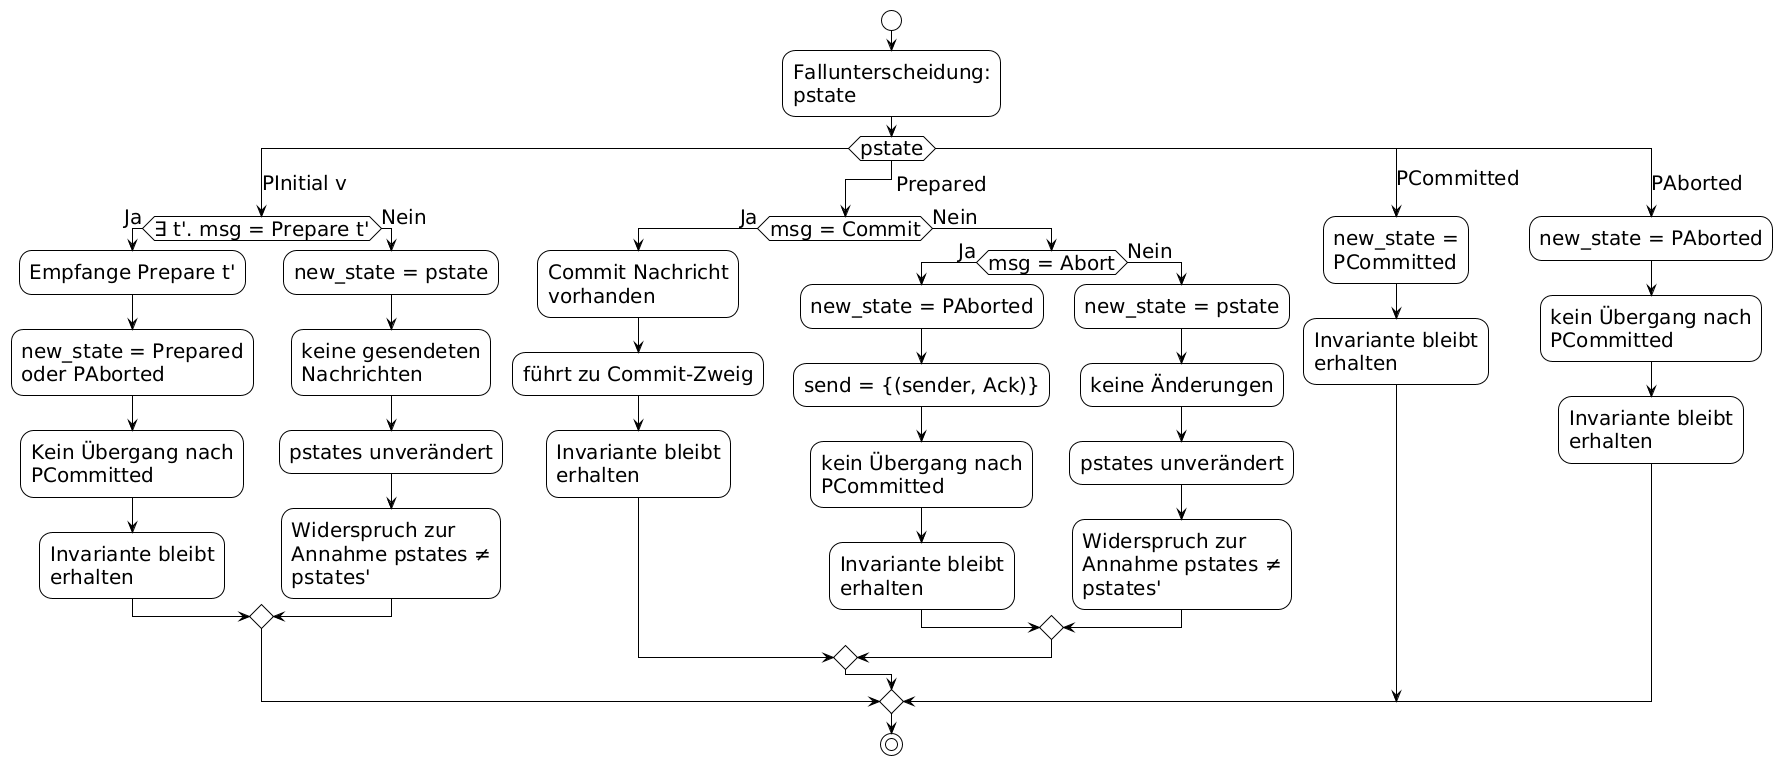
\includegraphics[width=1.0\textwidth]{Bilder/Beweisführung}
		\label{fig:beweisführung}
	\end{figure}
	
	Im gleichen Stile können die Fälle für eine Timeout- und Restart-Aktion gezeigt werden.
	
	\newpage
	\subsection{Beweis der einheitlichen Zustimmung}
	Die Beweisführung der einheitlichen Zustimmung erfolgt mittels der gleichen Invarianten analog zum Modell von Kleppmann. Aufgrund von besserer Übersichtlichkeit, werden folgende Definitionen eingeführt, um anzugeben ob sich ein Prozess im Committed- oder Aborted-Zustand befindet:
	
	\thyIoaAc{10}{18}
	
	Diese Definitionen erlauben eine analoge Formulierung der folgenden Lemmas im Vergleich zum Modell von Kleppmann. Die Beweisführung bleibt semantisch unverändert:
	
	\thyIoaAc{20}{25}
	
	\thyIoaAc{68}{73}
	
	\thyIoaAc{107}{111}
	
	\newpage
	\section{Vergleich der Modellierungsansätze}
	Da nun das Zwei-Phasen-Commit-Protokoll in beiden Frameworks implementiert und die zentrale Eigenschaft der einheitlichen Zustimmung bewiesen wurde, können darauf aufbauend die verwendeten Modellierungsansätze detailliert gegenübergestellt werden.
	
	\subsection{Erarbeitung der Vergleichskriterien}
	Für einen aussagekräftigen Vergleich werden rein quantitative Metriken, wie etwa die Anzahl der Beweiszeilen, bewusst vernachlässigt, da diese stark von individuellen Modellierungsentscheidungen abhängen und nicht zwingend die Qualität eines Ansatzes widerspiegeln.
	Stattdessen fokussiert sich dieser Vergleich auf qualitative Kriterien, welche maßgeblich bestimmen, wie skalierbar, anwendbar und nutzerfreundlich ein Framework in der Praxis ist:
	
	Ein flexibles Framework kann zur Modellierung verschiedenster Systemarchitekturen und Fehlermodelle genutzt werden, anstatt den Nutzer in vorgefertigte Schablonen zu zwingen \cite{efFr}. Modularität wiederum ist entscheidend für das Prinzip 'Teile und Herrsche': Erlaubt ein Framework die Kapselung und Wiederverwendung von Systemkomponenten, lassen sich auch gigantische Zustandsräume beherrschen.
	
	Die Nähe zur Spezifikation ist essenziell für die Fehlerprävention. Wenn eine Formalisierung zu weit vom eigentlichen Algorithmus abstrahiert ist, können beim Übergang unbemerkt semantische Fehler entstehen. Es ist von Vorteil, wenn eine Formalisierung nicht zu weit vom eigentlichen Algorithmus abweicht, da andernfalls leichter unbemerkt semantische Fehler entstehen können.
	Dabei hilft ein Vergleich der letztendlichen Darstellung des Zwei-Phasen-Commit-Protokolls, um ein Verständnis über die Ähnlichkeit beider Frameworks zueinander aufzubauen.
	
	Weiterhin hilft die Beweisstruktur und der Beweisaufwand die praktische Nutzbarkeit einzuschätzen. Ein mathematisch perfektes Modell bietet wenig Nutzen, wenn die formale Verifikation selbst einfachster Eigenschaften sehr aufwändig ist. 
	
	Ein gutes Framework sollte über reine Safety-Garantien hinausgehen. Die Unterstützung von Liveness-Eigenschaften ist ein wichtiges Kriterium, da sie den Nachweis ermöglicht, dass ein verteiltes System tatsächlichen Fortschritt macht und nicht etwa in einem Deadlock verharrt \cite{kleppmannblog}.
	
	Der Einstieg in die formale Verifikation ist zumeist komplex. Dokumentationen und existierende Code-Beispiele sind dabei sehr hilfreich, um diese Einstiegshürde zu senken. Zudem sollte Isabelles Automatisierung vom Framework gut genutzt werden können um den Beweissprozess drastisch zu verkürzen und zu vereinfachen.
	 
	\subsection{Flexibilität und Modularität}
	Die beiden Frameworks verfolgen bei der Flexibilität fast entgegengesetzte Philosophien. Die Ausführungssemantik im Modell von Kleppmann ist sehr streng: Es ist fest vorgegeben, dass immer exakt ein Prozess ein Event ausführt \cite{kleppmannblog}. Globale Events sind nicht ohne Umwege möglich und die Struktur des Netzwerks ist durch den globalen Nachrichtenpool starr vorgegeben.
	Das IOA-Framework hingegen zeichnet sich durch seinen inhärenten Nicht-Determinismus aus. Auch die Netzwerkkanäle müssen selbst modelliert werden. Diese enorme Flexibilität erlaubt es, verschiedenste Netzwerktopologien oder spezifische Kommunikationsmuster präzise abzubilden.
	
	Das Modell von Kleppmann sieht Modularität nativ nicht vor \cite{lynchbook}. Zwar lassen sich Übergangsfunktionen manuell kombinieren, wie es bei Koordinator und Teilnehmer gemacht wurde, das System bleibt jedoch tendenziell eine starre monolithische Einheit. 
	Das formale IOA Modell von Lynch hingegen hat die Komposition als einen Hauptbestandteil \cite{lynchbook}, welche auch nativ vom Isabelle-Framework unterstützt wird. Eine Einschränkung besteht lediglich darin, dass das Framework eine Komposition von unendlich vielen IOA nicht nativ unterstützt und wie bei dem Teilnehmer-IOA eigenständig durchgeführt werden muss.
	
	\subsection{Ähnlichkeit Formalisierung vs Algorithmus}
	Im Modell von Kleppmann konnten die Übergangsfunktionen fast vollständig und direkt der Protokollspezifikation nachempfunden werden, weshalb sich in diesem Modell, Formalisierung und Algorithmus/Spezifikation sehr ähneln.
	Im IOA-Framework sind die Übergangsfunktionen selbst zwar ebenfalls ähnlich, jedoch ist die daraus resultierende Übergangsrelation deutlich abstrakter, da sie für die Darstellung von Nicht-Determinismus genutzt wird. Dies sorgt für eine stärkere Abstraktion vom ursprünglichen Algorithmus.
	\subsection{Formalisierung des Zwei-Phasen-Commit-Protokolls}
	Beim Modell von Kleppmann orientieren sich die Übergangsfunktionen stark an der Spezifikation der Protokollbeschreibung. Um die Invarianten nicht unnötig umständlich formulieren zu müssen, wurde für die Zustände von Koordinator und Teilnehmern ein gemeinsamer Datentyp verwendet.
	
	Im IOA-Framework ist der Modellierungsaufwand merklich höher: Neben den Übergangsfunktionen, die ähnlich direkt aus der Protokollspezifikation hervor gingen, müssen Aktions-Signaturen definiert und explizite Übergangsrelationen generiert werden. Ein wesentlicher Faktor für den Mehraufwand ist zudem die explizite Modellierung der Netzwerkkanäle als eigener IOA und die anschließende Komposition aller Teilautomaten.
	\subsection{Beweisstruktur}
	Die grundsätzliche Struktur der Beweise ähnelt sich stark:
	Der Beweis von Invarianten erfordert in beiden Frameworks eine Induktion über die Ausführung in Verbindung einer anschließenden Fallunterscheidung, wer den Übergang getätigt hat gefolgt von ausgeführter Aktion/ ausgeführtem Event und aktuellem Zustand des ausführenden Prozesses.
	Da dass Modell von Kleppmann deutlich strenger ist entfallen viele Zwischenschritte, die beim potenziell Nicht-Deterministischen IOA-Modell nötig waren.
	Der Beweis der einheitlichen Zustimmung ist in beiden Modellen nahezu identisch.
	\subsection{Beweisaufwand}
	Der Beweisaufwand korreliert stark mit der Flexibilität des Frameworks. Das Modell von Kleppmann ist deterministischer und strukturell weniger flexibel, was tendenziell zu deutlich kürzeren und direkteren Beweisen führt.
	
	Das IOA Modell hingegen ist inhärent nicht-deterministisch und in seiner Struktur enorm flexibel. Diese schwachen strukturellen Vorgaben erfordern mehr manuellen Aufwand, da die Beweisführung direkter gelenkt werden muss.
	\subsection{Nachweis von Liveness-Eigenschaften}
	Während Safety-Eigenschaften, wie einheitliche Zustimmung garantieren, dass 'nichts Ungewünschtes' passiert, stellen Liveness-Eigenschaften sicher, dass 'irgendwann das Erwünschte' passiert \cite{kleppmannbook}. Dies steht oft in engem Zusammenhang mit Annahmen über Fairness oder das Netzwerk. 
	
	Kleppmann macht bewusst keine Annahmen über Fairness, da diese oft zu fallspezifisch sind. Dadurch unterstützt das Modell von Kleppmann Fairness nicht nativ. Lässt sich aber über eigene Annahmen in Kombination mit der Event-Semantik gut abbilden. 
	
	Das IOA Modell von Lynch hingegen unterstützt Fairness grundlegend. Auch das verwendete Framework bietet grundlegende Funktionalität für Fairness. Da das Netzwerk bei IOA als eigenständiger Automat modelliert werden muss, können realistische Netzwerkannahmen direkt über die Komposition in das Gesamtsystem integriert werden.
	
	\newpage
	\subsection{Automatisierungsgrad in Isabelle}
	Ein großer Vorteil der computergestützten Beweisführung in Isabelle ist die Automatisierung durch Hilfen wie 'Sledgehammer' \cite{semantics}. 
	Kleppmanns Framework ist klein und auf das Wesentliche reduziert, was sehr gut mit Isabelles Automatisierung einher geht. Sledgehammer bietet hier gute Unterstützung. 
	
	Im IOA-Framework fällt es Sledgehammer aufgrund der vielen, tief verschachtelten Definitionen schwer, eigenständig Beweise zu finden. Oft müssen Definitionen erst manuell expandiert werden. Dies führt außerdem dazu, dass die zu zeigenden Aussagen deutlich größer und unübersichtlicher werden, weshalb für das IOA-Framework weitaus öfter manuell Hilfslemmata, insbesondere für Übergänge innerhalb von Kompositionen, geschrieben werden müssen.
	\subsection{Dokumentation zur Nutzung der Frameworks}
	Gute Beweisbeispiele und Dokumentationen sind essenziell für den Einstieg in das jeweilige Framework.
	Für das Modell von Kleppmann existiert eine zugängliche Demonstration von Kleppmann selbst, in der ein einfacher Konsensalgorithmus formalisiert wird \cite{kleppmannblog}. Der Code ist online verfügbar und leicht verständlich \cite{kleppmanncode}. Bei sehr komplexen Systemen kann es jedoch passieren, dass man aufgrund fehlender Werkzeuge 'kreativ' werden muss, um das Protokoll abzubilden. 
	
	Da I/O-Automaten ein theoretisch weit verbreitetes Modell sind, gibt es viel konzeptionelle Literatur. Zwar existieren auch Formalisierungsbeispiele für ähnliche IOA-Frameworks (etwa von Nipkow selbst), diese zeigen jedoch oft wenig konkreten Code zur Beweisführung, was die Einarbeitung in die praktische Nutzung erschwert \cite{ioaOldFramework} \cite{ioaHolCF}.
	
	\newpage
	\section{Schluss}
	Die Verwendung formaler Beweismethoden zum Nachweis von Korrektheit verteilter Systeme ist besonders wichtig, da solche Systeme oft zu komplex sind und Fehler teilweise lange unentdeckt bleiben \cite{kleppmannblog}. Die Darstellung eines solchen verteilten Systems kann über eine Vielzahl an Modellen geschehen.
	
	In dieser Arbeit wurde das Zwei-Phasen-Commit-Protokoll in Isabelle mithilfe zweier unterschiedlicher Frameworks modelliert und die Eigenschaft der einheitlichen Zustimmung bewiesen. Dabei wurden typische Fehlerquellen verteilter Systeme wie Nachrichtenverlust, Duplikation oder Prozessausfälle berücksichtigt.
	
	Anschließend erfolgte ein Vergleich beider Frameworks sowie der Modellierung und Beweisführung. Der Vergleich zeigt, dass beide Ansätze grundsätzlich geeignet sind, verteilte Systeme formal zu beschreiben und deren Korrektheit zu verifizieren, jedoch unterschiedliche Schwerpunkte setzen.
	Das Modell von Kleppmann bietet eine praxisnahe und einfache Sicht auf verteilte Systeme, mit der die Automatisierung in Isabelle voll ausgenutzt werden kann.
	Das IOA-Framework stammt von einem weit verbreiteten mathematischen Modell, das von Nancy A. Lynch und Mark R. Tuttle erstmals eingeführt wurde. Es überzeugt besonders mit seiner Flexibilität in Modellierung und Komposition mehrerer IOA, was den Wiederverwendungswert aber auch die Komplexität von Beweisen in diesem Modell erhöht.
	
	Ein wesentlicher Unterschied zeigt sich zudem in der Unterstützung weicherer Eigenschaften. Während das Modell von Kleppmann primär auf Safety-Eigenschaften ausgelegt ist und Fairnessannahmen nur indirekt integriert werden können, bietet das IOA-Modell hierfür bereits konzeptionelle Grundlagen. Dadurch eignet es sich besser für die Analyse von Liveness-Eigenschaften und langfristigem Systemverhalten. Zusätzlich verfügt das Modell von Kleppmann über eine gut dokumentierte beispielhafte Nutzung des Frameworks, was den Einstieg damit deutlich vereinfacht. Gleichzeitig können die von Isabelle bereitgestellten Hilfen wie 'Sledgehammer' deutlich besser mit dem Modell von Kleppmann als mit dem IOA-Modell genutzt werden.
	
	Zusammenfassend lässt sich sagen, dass sich beide Ansätze dazu eignen die Korrektheit verteilter Systeme auch unter schwierigen Bedingungen zuverlässig nachzuweisen. Gleichzeitig hat die Wahl der Modellierungsmethode einen erheblichen Einfluss auf die Komplexität der Verifikation und sollte bewusst getroffen werden.
	
	\newpage
	\section{Quellen}
	\printbibliography
\end{document}